\documentclass{article}
\usepackage{tikz}
\usetikzlibrary{shapes,arrows,positioning}

\begin{document}
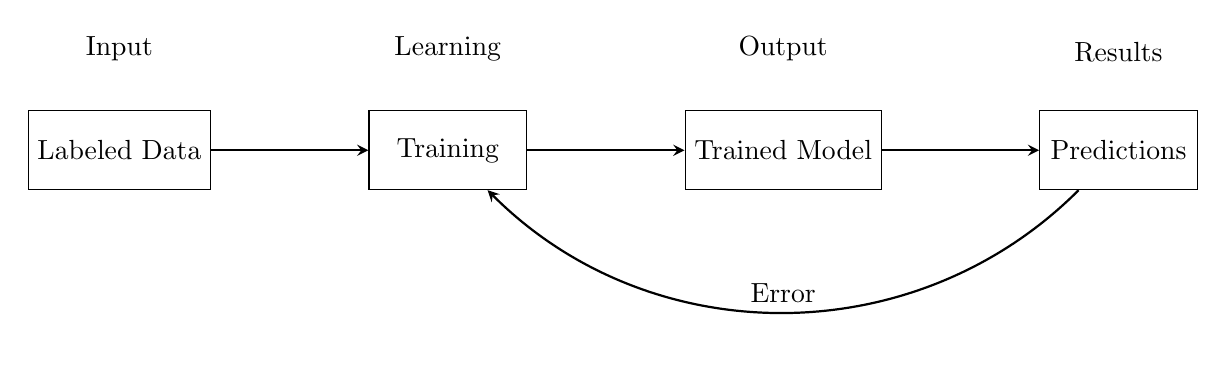
\begin{tikzpicture}[
    node distance=2cm,
    block/.style={rectangle, draw, minimum width=2cm, minimum height=1cm},
    arrow/.style={thick,->,>=stealth}
]

% Input data
\node[block] (data) {Labeled Data};
\node[block, right=of data] (train) {Training};
\node[block, right=of train] (model) {Trained Model};
\node[block, right=of model] (predict) {Predictions};

% Arrows
\draw[arrow] (data) -- (train);
\draw[arrow] (train) -- (model);
\draw[arrow] (model) -- (predict);

% Feedback loop
\draw[arrow] (predict) to[bend left=45] node[above] {Error} (train);

% Labels
\node[above=0.5cm of data] {Input};
\node[above=0.5cm of train] {Learning};
\node[above=0.5cm of model] {Output};
\node[above=0.5cm of predict] {Results};

\end{tikzpicture}
\end{document} 